
%(BEGIN_QUESTION)
% Copyright 2009, Tony R. Kuphaldt, released under the Creative Commons Attribution License (v 1.0)
% This means you may do almost anything with this work of mine, so long as you give me proper credit

The process trend shown below reveals a controller's response to the process variable signal and the setpoint.  Based on what you see in this trend, determine whether the controller is direct or reverse acting, and also whether it implements a P-only, I-only, P+I, I+D, or P+D control algorithm.

$$\includegraphics[width=15.5cm]{i03770x01.eps}$$

\vskip 20pt \vbox{\hrule \hbox{\strut \vrule{} {\bf Suggestions for Socratic discussion} \vrule} \hrule}

\begin{itemize}
\item{} A useful problem-solving technique to apply here is working the problem {\it backwards}: ask youself what the output trend would look like for each action (P, I, D) and then see what the given output trend most resembles.
\item{} Integral and Derivative control actions are often discernable from the {\it phase shift} they introduce between the output and PV ``waves''.  Do you see any evidence of such phase shift in this trend?  If so, which action (I or D) does that phase shift suggest?
\end{itemize}

\underbar{file i03770}
%(END_QUESTION)





%(BEGIN_ANSWER)

This is a {\it reverse-acting}, {\it proportional + derivative} controller.


%(END_ANSWER)





%(BEGIN_NOTES)

A significant clue to determining this controller possesses derivative action is to note that the peak of the output wave {\it leads} the peak of the input (PV) wave.

%INDEX% Control: determining P, I, D from graph of controller response

%(END_NOTES)


